\documentclass[lualatex,ja=standard]{beamer}

\usepackage{luatexja-fontspec}
\usepackage{amssymb}
\usepackage{amsmath}
\usepackage{tikz}
\usepackage{pgf}
\usepackage[]{hyperref}
\usepackage{graphicx}
\usepackage{float}


\author{小森理央}
\title{可換砂山モデル}
\date{2023年2月1日}

\begin{document}

\begin{frame}
 \titlepage
\end{frame}


\begin{frame}{パターン形成(正方格子)}

\only<1>{
\begin{center}
 \begin{figure}[H]
  \begin{center}
   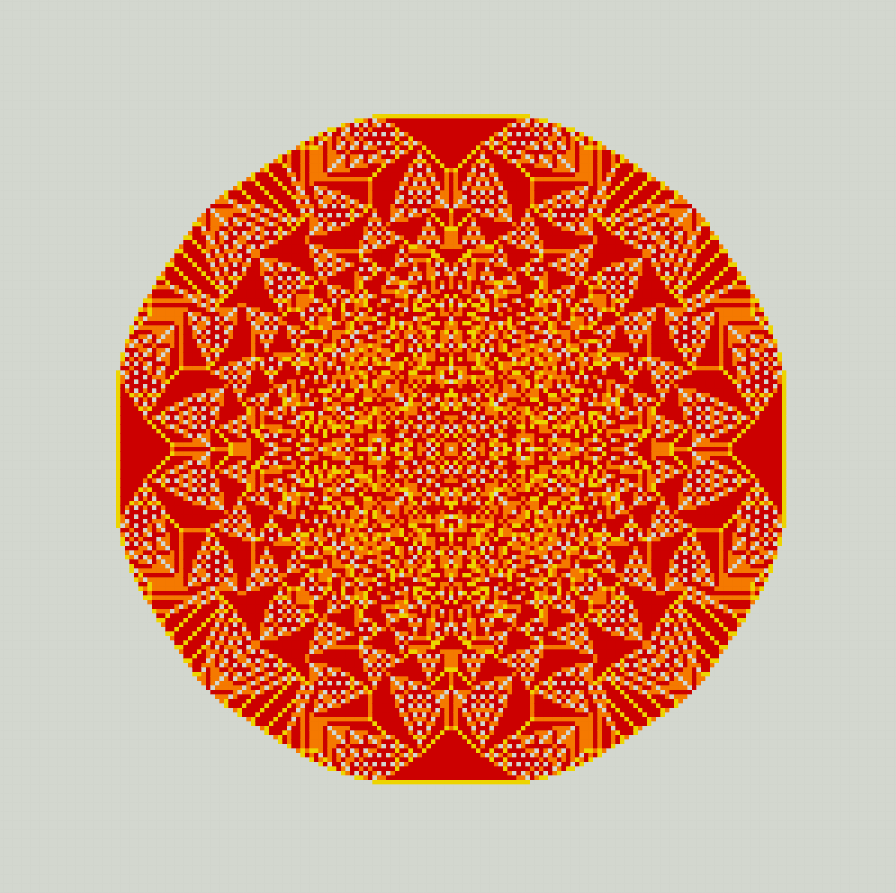
\includegraphics[bb=0 0 896 893,clip,width=8cm]{figures/onepoint40000.png}
  \end{center}
  \caption{1点に砂粒を投下して安定化させた様子:4万粒}
  \label{fig:onePoint40000}
 \end{figure}
\end{center}
} 

\only<2>{
\begin{center}
 \begin{figure}[H]
  \begin{center}
   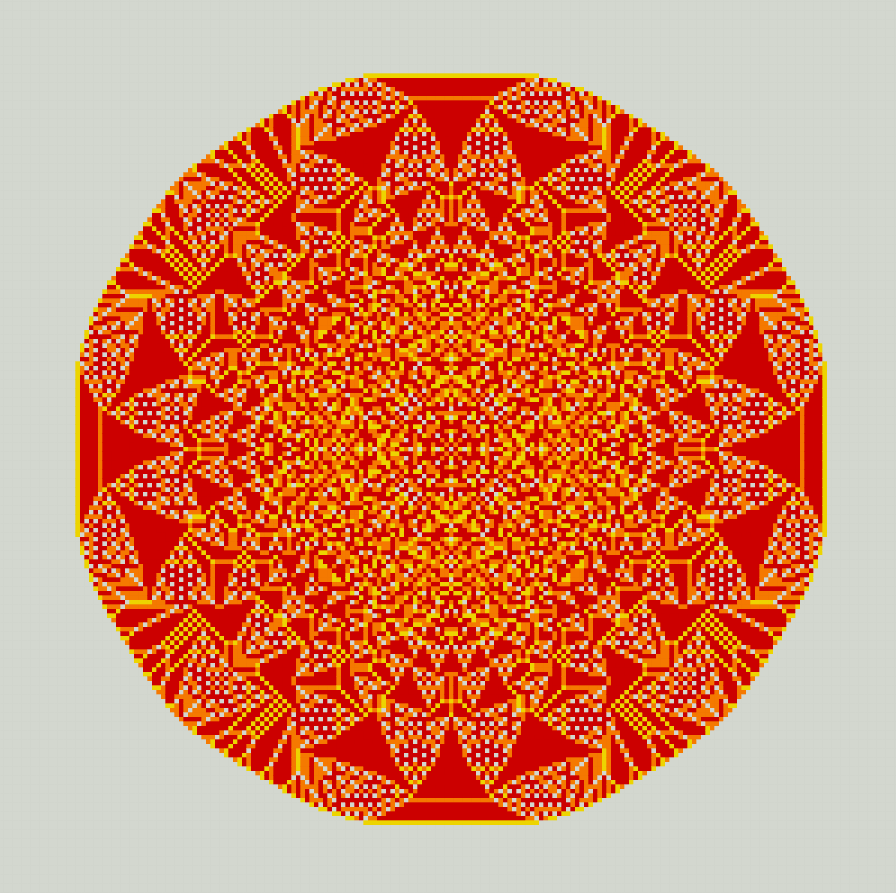
\includegraphics[bb=0 0 896 893,clip,width=8cm]{figures/onePoint50000.png}
  \end{center}
  \caption{1点に砂粒を投下して安定化させた様子:5万粒}
 \end{figure}
\end{center}
}

\only<3>{
\begin{center}
 \begin{figure}[H]
  \begin{center}
   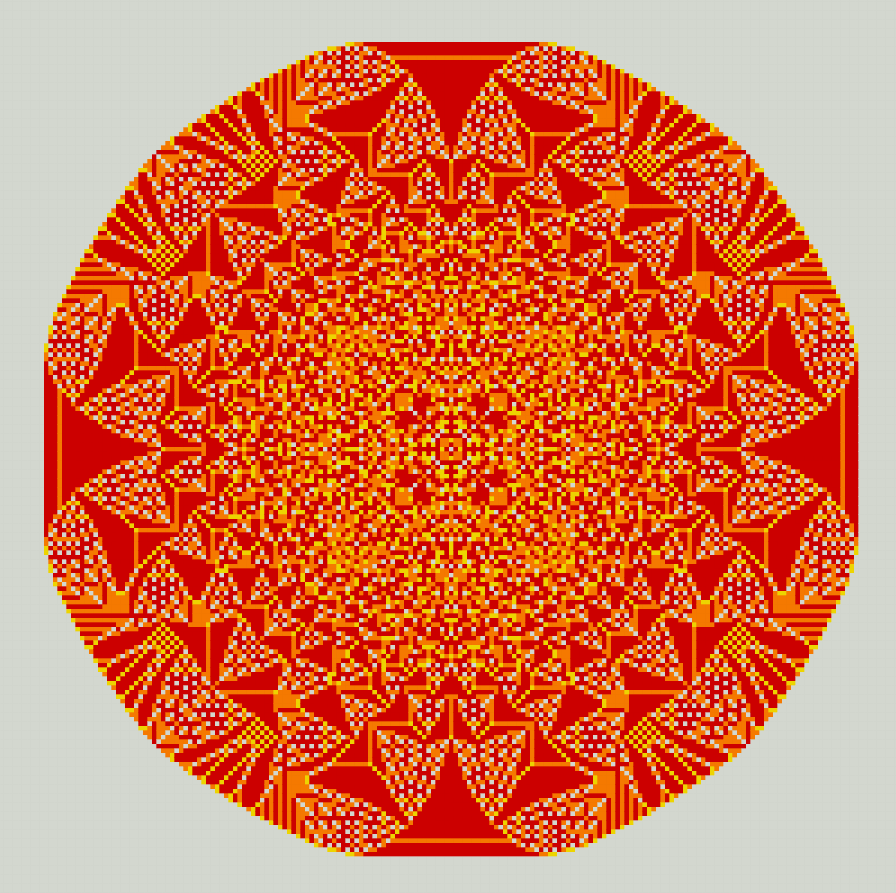
\includegraphics[bb=0 0 896 893,clip,width=8cm]{figures/onePoint6000.png}
  \end{center}
  \caption{1点に砂粒を投下して安定化させた様子:6万粒}
 \end{figure}
\end{center}
}

\only<4>{
\begin{center}
 \begin{figure}[H]
  \begin{center}
   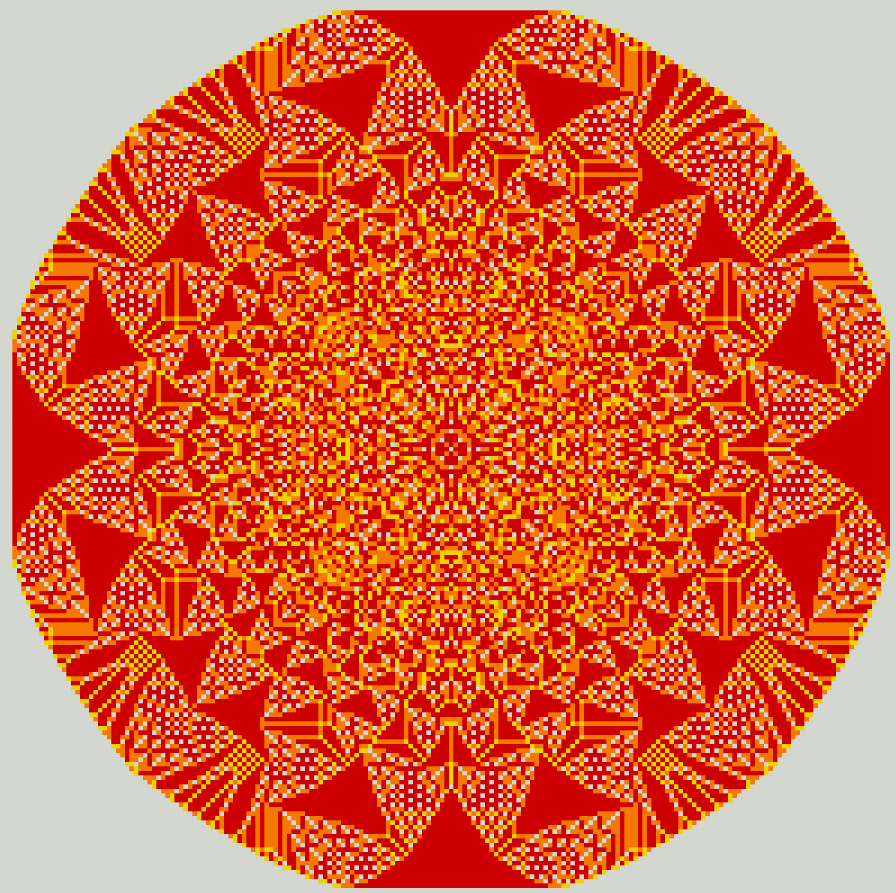
\includegraphics[bb=0 0 896 893,clip,width=8cm]{figures/onePoint70000.png}
  \end{center}
  \caption{1点に砂粒を投下して安定化させた様子:7万粒}
  \label{fig:onePoint70000}
 \end{figure}
\end{center}
}

\end{frame}

\begin{frame}{ペンローズタイル張り}
ペンローズタイル張りはノーベル物理学賞受賞者の
ロジャー・ペンローズ氏が発見した準周期性と呼ばれる
特徴を持つ二次元平面のタイル張りである。

\end{frame}

\begin{frame}{構成法1}
	    \begin{center}
	     \begin{figure}[H]
	      \begin{center}
	       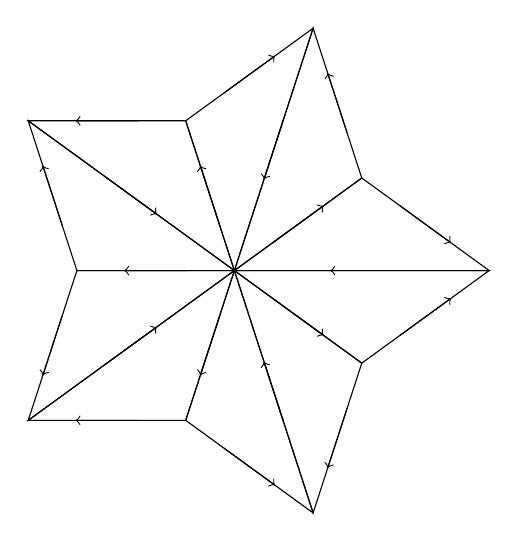
\begin{tikzpicture}[scale=2]
		\draw[->,>=latex] (0,0) -- ({2*cos(36)},0) -- ({cos(36)},{sin(36)})--cycle;
		\draw[->,>=latex] (0,0) -- ({2*cos(36)},0) -- ({cos(36)},{-sin(36)})--cycle;
		\draw[->] ({cos(36)+0.2},0) -- ({cos(36)-0.2},0);
		\draw[->] ({cos(36)*0.3},{sin(36)*0.3}) -- ({cos(36)*0.7},{sin(36)*0.7});
		\draw[->] ({cos(36)},{sin(36)}) ++ ({cos(36)*0.3},{-sin(36)*0.3}) -- ++ ({cos(36)*0.4},{-sin(36)*0.4});
		\draw[->] ({cos(36)},{-sin(36)}) ++ ({cos(36)*0.3},{sin(36)*0.3}) -- ++ ({cos(36)*0.4},{sin(36)*0.4});
		\foreach \i in {1,...,4}{
		\begin{scope}[rotate={\i*72}]
		\draw[->,>=latex] (0,0) -- ({2*cos(36)},0) -- ({cos(36)},{sin(36)})--cycle;
		\draw[->,>=latex] (0,0) -- ({2*cos(36)},0) -- ({cos(36)},{-sin(36)})--cycle;
		\draw[->] ({cos(36)+0.2},0) -- ({cos(36)-0.2},0);
		\draw[->] ({cos(36)*0.3},{sin(36)*0.3}) -- ({cos(36)*0.7},{sin(36)*0.7});
		\draw[->] ({cos(36)},{sin(36)}) ++ ({cos(36)*0.3},{-sin(36)*0.3}) -- ++ ({cos(36)*0.4},{-sin(36)*0.4});
		\draw[->] ({cos(36)},{-sin(36)}) ++ ({cos(36)*0.3},{sin(36)*0.3}) -- ++ ({cos(36)*0.4},{sin(36)*0.4});
		\end{scope}
		}
	       \end{tikzpicture}
	      \end{center}
	     \end{figure}
	    \end{center}
\end{frame}


\begin{frame}{構成step2(細分)}
	    \begin{center}
	     \begin{figure}[H]
	      \begin{center}
	       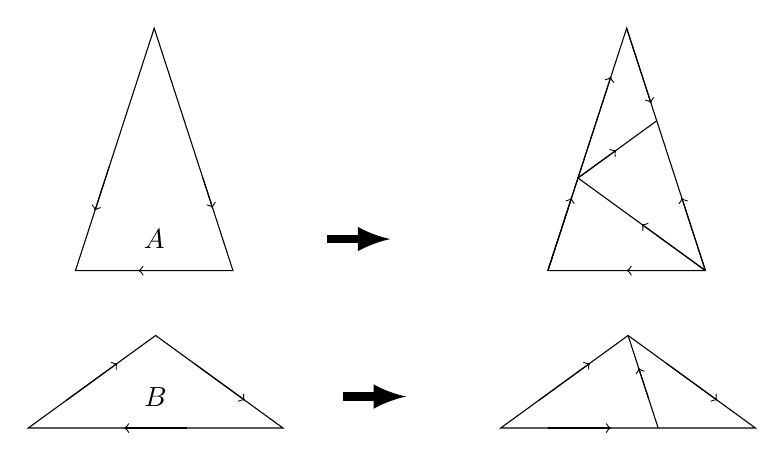
\begin{tikzpicture}[scale=2]
		\draw[->,>=latex] (0,0) -- ({2*cos(36)},0) -- ({cos(36)},{sin(36)})--cycle;
		\draw[->] ({cos(36)+0.2},0) -- ({cos(36)-0.2},0);
		\draw[->] ({cos(36)*0.3},{sin(36)*0.3}) -- ({cos(36)*0.7},{sin(36)*0.7});
		\draw[->] ({cos(36)},{sin(36)}) ++ ({cos(36)*0.3},{-sin(36)*0.3}) -- ++ ({cos(36)*0.4},{-sin(36)*0.4});
		\draw ({cos(36)},0.2) node {$B$};
		\draw[line width = 3, ->, >=latex](2,0.2) -- (2.4,0.2);
		\begin{scope}[xshift=3cm]
		\draw[->,>=latex] (0,0) -- ({2*cos(36)},0) -- ({cos(36)},{sin(36)})--cycle;
		 \draw[] (1,0) -- ({cos(36)}, {sin(36)});
		 \draw[->] (0.3,0) -- (0.7,0);
		 \draw[->] ({0.3*cos(36)},{0.3*sin(36)}) -- ({0.7*cos(36)},{0.7*sin(36)});
		 \draw[->] ({cos(36)},{sin(36)}) ++ ({cos(36)*0.3},{-sin(36)*0.3}) -- ++ ({cos(36)*0.4},{-sin(36)*0.4});
		 \draw[->] (1,0) ++ ({cos(108)*0.2},{sin(108)*0.2}) -- ++({cos(108)*0.2},{sin(108)*0.2});
		\end{scope}
		\begin{scope}[yshift=1cm,xshift=0.3cm]
		 \draw (0,0) --  (1,0) -- ({1/2},{tan(72)/2}) -- cycle;
		 \draw[->] ({cos(72)*0.7},{sin(72)*0.7}) -- ({cos(72)*0.4},{sin(72)*0.4});
		 \draw[->] ({1/2},{tan(72)/2}) ++ ({cos(72)},{-sin(72)}) -- ++({cos(72)*0.2},{-sin(72)*0.2});
		 \draw[->] (0.7,0) -- (0.4,0);
		 \draw[line width = 3, ->, >=latex](1.6,0.2) -- ++(0.4,0);
		 \draw ({1/2)},0.2) node {$A$};
		\begin{scope}[xshift=3cm]
		 \draw (0,0) --  (1,0) -- ({1/2},{tan(72)/2}) -- cycle;
		 \draw[->] (1,0) -- ++({-1/2*0.3},{tan(72)/2*0.3});
		 \draw[->] (1,0) -- (0.5,0);
		 \draw[->] (0,0) -- ++({1/2*0.3},{tan(72)/2*0.3});
		 \draw[->] (0,0) -- ++({1/2*0.8},{tan(72)/2*0.8});
		 \draw (1,0) -- ++({cos(144)},{sin(144)}) -- ({1+cos(108)},{sin(108)});
		 \draw[->] (1,0) -- ++({cos(144)*0.5},{sin(144)*0.5});
		 \draw[->] ({1/2},{tan(72)/2}) -- ++({cos(72)*0.5},{-sin(72)*0.5});
		 \draw[->] ({1+cos(144)},{sin(144)}) -- ++ ({0.3*cos(36)},{0.3*sin(36)});
		\end{scope}
		\end{scope}

	       \end{tikzpicture}
	      \end{center}
	     \end{figure}
	    \end{center}
 \end{frame}

 \begin{frame}{構成法step3(拡大)}
  	    すべての三角形を原点を中心に$\frac{1+\sqrt{5}}{2}$倍相似拡大する。
	    (すべての頂点の原点からの距離が$\frac{1+\sqrt{5}}{2}$倍される。)
	    この結果得られる三角形はすべてタイプ$A$か$B$のいずれかである。
 \end{frame}

 \begin{frame}{構成法step3(貼り合わせ)}
	    底辺で接する2つの2等辺三角形を貼り合わせひし形タイル張りを作る。
 \end{frame} 
\end{document}